\section{Обзор исследуемых методов}
\label{sec:theory}

\subsection{Общее описание метода решения нелинейных уравнений}
Обычно решение уравнений вида~\ref{intro:formula_def} осуществляется используя численные методы, которые при этом разбивают процесс решения таких уравнений на два этапа~\cite[стр. 48]{vich_mat}:
\begin{enumerate}
	\item Приближенное определение местоположения, характер и выбор интересующего нас корня;
	\item \label{theory:steps_second} Вычисление выбранного корня с заданной точностью $\varepsilon$.
\end{enumerate}

Первый этап такого решения решается графическим способом: на отрезке $[a,b]$ вычисляется таблица значений функции с некоторым шагом $h$, строится её график и определяются интервалы $(\alpha_i, \beta_i)$ длиной $h$, на которых располагаются корни уравнения. 

На рисунке~\ref{fig:theory:graph} представлены три наиболее чаще встречающихся ситуации во время нахождения таких корней:
\begin{enumerate}
	\item кратный корень: $f'(x_1^*)=0,\ f(\alpha_1)\cdot f(\beta_1) > 0$;
	\item простой корень: $f'(x_2^*)\neq 0,\ f(\alpha_2)\cdot f(\beta_2)<0$;
	\item вырожденный корень: $f'(x_3^*)$ не существует, $f(\alpha_3)\cdot f(\beta_3)>0$.
\end{enumerate}
\begin{figure}[ht]
	\centering
	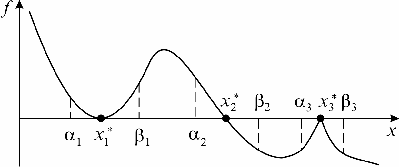
\includegraphics{attachments/theory_graph}
	\caption{ График некой функции, показывающий наиболее частые ситуации}
	\label{fig:theory:graph}
\end{figure}

Как видно на рисунке~\ref{fig:theory:graph}, значение корней в случаях ``а'' и ``б'' совпадает с точкой экстремума функции, и для нахождения таких корней можно воспользоваться
многочисленными методами поиска минимума функции.

На втором этапе вышеописанного процесса решения уравнений вычисление значения корня с заданной точностью осуществляется одним из так называемых ``итерационных методов''. Общей методологией заключается в том, что на интервале $(\alpha, \beta)$, где находится интересующий корень $x^*$, выбирается $m$ начальных значений $x_0, x_1,\dots,x_{m-1}$ (обычно $x_0 = \alpha, x_1 = \beta$), после чего последовательно находятся члены $(x_m, x_{m+1}, \dots, x_{n-1}, x_n)$ рекуррентной последовательности порядка $m$ по правилу $x_k = \varphi(x_{k-1}, \dots, x_{k-m})$ до тех пор, пока $\left|x_n - x_{n-1}\right|<\varepsilon$. Последнее $x_n$ выбирается в качестве приближённого значения корня ($x^* \approx x_n$).

\subsection{Метод простых итераций для уточнения значения корней уравнения}
Очень часто на практике встречается ситуация, когда уравнение вида~\ref{theory:steps_second} записано в виде, разрешённом относительно $x$~\cite[стр. 49]{vich_mat}:
\begin{equation}
	\label{eq:theory:solved_for}
	x=\varphi(x)
\end{equation}
Такой переход от записи~\ref{theory:steps_second} к записи~\ref{eq:theory:solved_for} можно осуществить множеством способов, например:
\begin{equation}
	\label{eq:theory:iter:solve}
	\varphi(x)=x+\Psi(x)f(x)
\end{equation}
\begin{explanation}
	где & $\Psi(x)$ & произвольная непрерывная знакопостоянная функция (часто достаточным является выбор $\Psi = \text{const}$).
\end{explanation}

В таком случае можно говорить, что корни уравнения~\ref{eq:theory:solved_for} также являются верными корнями уравнения~\ref{intro:formula_def}~\cite{vich_mat}.

Исходя из записи~\ref{eq:theory:solved_for}, члены рекуррентной последовательности в методе простых итераций вычисляются по закону
\begin{equation}
	x_k=\varphi(x_{k-1}),\, k=1,2,\dots
\end{equation}

Поскольку такая последовательность имеет порядок $m=1$, этот метод является одношаговым, поэтому для начала вычислений достаточно знать одно начальное приближение $x_0 = \alpha$ или $x_0 = \beta$, или $x_0=\frac{\alpha + \beta}{2}$.

Условием сходимости метода простой итерации, если $\varphi(x)$ дифференциируема, является выполнение неравенства $\left|\varphi'(\xi)\right|$ для любого 
\begin{equation}
	\label{eq:theory:iter:condition}
	\xi = (\alpha, \beta),\, x^*\in(\alpha, \beta)
\end{equation}

Минимальный интервал $(\alpha,\ \beta)$, для которого выполняется неравенство~\ref{eq:theory:iter:condition}, называется \textbf{областью сходимости}.

При соблюдении условия~\ref{eq:theory:iter:condition} метод сойдется, если начальное значение x0 выбрано в пределах области сходимости. В таком случае скорость убывания погрешности $\varepsilon_k = \left|x^* - k_k \right|$ к нулю в окрестности корня приблизительно такая же, как у геометрической прогрессии $\varepsilon_k\approx \varepsilon_{k-1}q$ со знаменателем $q\cong \left|\varphi'(x^*)\right|$, т.е. чем меньше $q$, тем быстрее сходимость, и наоборот.
Поэтому при переходе от~\ref{intro:formula_def} к~\ref{eq:theory:solved_for} функцию $\varphi(x)$ в~\ref{eq:theory:iter:solve} выбирают таким образом, чтобы было выполнено условие сходимости~\ref{eq:theory:iter:condition} для как можно большего интервала $(\alpha, \beta)$ и при этом с наименьшим значением $q$. Удачный выбор этих условий обеспечивает эффективность вычислений.

Блок-схема алгоритма простых итераций указана на рисунке~\ref{fig:theory:iter:algo}.
\begin{figure}[ht]
	\centering
	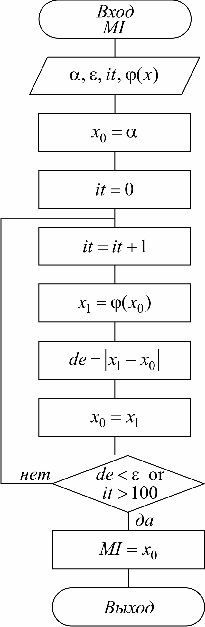
\includegraphics{attachments/theory_simple_iterations_algo}
	\caption{Алгоритм реализации метода простых итераций}
	\label{fig:theory:iter:algo}
\end{figure}

\subsection{Метод Ньютона}
Этот метод является модификацией метода простых и иногда называется методом касательных. Суть его в следующем: если $f(x)$ имеет непрерывную производную, тогда, выбрав в~\ref{eq:theory:iter:solve} $\Psi(x) = \frac{-1}{f'(x)}$, получится эквивалентное уравнение $x=x-\frac{f(x)}{f'(x)}=\varphi(x)$, в котором $q\cong \varphi'(x^*)\equiv 0$. Поэтому скорость сходимости рекуррентной последовательности метода Ньютона
\begin{equation}
	x_k=x_{k-1} -\frac{f(x_{k-1})}{f'(x_{k-1})}
	\label{eq:theory:newton:speed}
\end{equation}
вблизи корня очень большая, погрешность очередного приближения примерно равна квадрату погрешности предыдущего $\varepsilon_k \cong \left|\varphi''(x^*)\right| \varepsilon_{k-1}^2$.

Из~\ref{eq:theory:newton:speed} видно, что этот метод одношаговый ($m=1$), и для начала вычислений требуется задать одно начальное приближение $x_0$ из области сходимости, определяемой неравенством $f\cdot f'' / (f')^2<1$.  Этот метод позволяет находить как простые, так и кратные корни. Основной его недостаток – малая область сходимости и необходимость вычисления производной $f'(x)$.

\subsection{Метод секущих}
Этот метод является модификацией метода Ньютона, позволяющей избавиться от явного вычисления производной путём её замены приближённой формулой. Тогда вместо процесса~\ref{eq:theory:newton:speed} получаем
\begin{equation}
	x_k=x_{k-1} -\frac{f(x_{k-1})h}{f(x_{k-1}) -f(x_{k-1} - h) }=\varphi(x_{k-1})
\end{equation}
\begin{explanation}
	где & h & некоторый малый параметр метода, который подбирается из условия наиболее точного вычисления производной.
\end{explanation}

Метод является одношаговым и его условие сходимости при правильном выборе $h$ такое же, как у метода Ньютона.